\documentclass[11pt]{article}
\usepackage[margin=1.05in]{geometry}
\usepackage{amsmath,amssymb,bm}
\usepackage{booktabs}
\usepackage{siunitx}
\usepackage{tikz}
\usetikzlibrary{arrows.meta,positioning}
\usepackage{listings}
\usepackage{xcolor}
\usepackage[colorlinks=true,linkcolor=blue,citecolor=blue,urlcolor=blue]{hyperref}

\newcommand{\ud}{\,\mathrm{d}}
\newcommand{\vect}[1]{\bm{#1}}
\newcommand{\file}[1]{\texttt{#1}}

\lstset{basicstyle=\ttfamily\footnotesize, frame=single, framesep=4pt,
        backgroundcolor=\color{gray!6}, columns=fullflexible,
        breaklines=true, showstringspaces=false}
\tikzset{
  stage/.style={draw, rounded corners=2pt, align=center, font=\small,
                minimum height=8mm, inner xsep=5pt, fill=orange!7},
  data/.style={draw, align=center, font=\scriptsize\ttfamily, fill=yellow!10,
               minimum height=7mm, inner xsep=4pt},
  fl/.style={-{Stealth[length=2mm]}, thick},
}

\title{Elliptic $\to$ GEO Minimum-Fuel Transfer: \\
Problem, Formulation, Discretization, and How to Run It}
\author{Michael Casey}
\date{July 26, 2026}

\begin{document}
\maketitle

\begin{abstract}
A working guide to the direct (collocation) solution of the minimum-fuel
low-thrust transfer from an elliptic orbit to GEO --- the two-body benchmark of
Haberkorn, Martinon and Gergaud, reproduced here with our own machinery across
a thrust ladder from \SI{10}{\newton} down to \SI{0.1}{\newton}. Covers the
optimal control problem, why it is posed in modified equinoctial elements with
true longitude as the independent variable, the discretization, the pipeline,
and how to run it. Derivations and the per-rung operational detail live in the
companion documents; this is the map.
\end{abstract}

\tableofcontents

%=======================================================================
\section{The transfer problem}
%=======================================================================

A spacecraft on a highly elliptic orbit ($P_0=\SI{11625}{\kilo\meter}$,
$e=0.75$, $i=\ang{7}$) must reach GEO using continuous low thrust, minimizing
propellant. Wet mass \SI{1500}{\kilo\gram}, $I_{sp}=\SI{2000}{\second}$. The
benchmark fixes the horizon at
\begin{equation}
t_f \;=\; c_{t_f}\cdot t_{f,\min}(T_{\max}),
\qquad c_{t_f}=1.5 ,
\end{equation}
i.e.\ each thrust level gets its own minimum-time anchor and the horizon is a
fixed multiple of it. As thrust falls the transfer stretches over more and more
revolutions --- from roughly seven at \SI{10}{\newton} to hundreds at
\SI{0.1}{\newton} --- and it is that growth, not the thrust value itself, that
makes the deep rungs hard.

%=======================================================================
\section{The optimal control problem}
%=======================================================================

\subsection{Why modified equinoctial elements}

Integrating Cartesian state over hundreds of revolutions is a losing
proposition: the fast angle dominates, and the mesh must resolve every
revolution of an orbit that is barely changing. Modified equinoctial elements
(MEE) separate the slow shape variables from the fast angle:
\[
\vect{x}_{\text{slow}} = \big(P,\ e_x,\ e_y,\ h_x,\ h_y\big),
\qquad \text{fast angle} = L \ (\text{true longitude}),
\]
with mass $m$ carried alongside. MEE are free of the singularities that afflict
classical elements at zero eccentricity and zero inclination, which matters
because the transfer ends at GEO --- circular and equatorial, exactly where
those singularities sit.

\subsection{Longitude as the independent variable}

The decisive move is to integrate in $L$ rather than $t$. The slow elements
evolve gently in $L$, so a mesh uniform in $L$ is well-matched to the dynamics
across hundreds of revolutions, and time becomes a state:
\begin{equation}
\frac{\ud \vect{x}}{\ud L} \;=\; \frac{\ud \vect{x}/\ud t}{\dot L},
\qquad
\frac{\ud t}{\ud L} \;=\; \frac{1}{\dot L}.
\end{equation}
The Gauss variational equations supply $\ud\vect{x}/\ud t$ in terms of the
thrust acceleration resolved in the RTN frame, $\vect{a}=\frac{T_{\max}}{m}s\,
\vect{\beta}$ with $\|\vect{\beta}\|=1$ and throttle $s\in[0,1]$.

\subsection{The free longitude span}

How much longitude does the transfer take? That is not known in advance --- it
is essentially the revolution count, which is part of the answer. So the total
span
\begin{equation}
\Delta L \;=\; L_f - L_0
\end{equation}
is itself a \emph{decision variable}, with the normalized independent variable
$\sigma\in[0,1]$ and $L(\sigma)=L_0+\sigma\,\Delta L$.

This is the structural counterpart of the CR3BP campaigns' Sundman
$\tau_f$ --- and the comparison is instructive. Here $\Delta L$ is free, so the
revolution count can grow, which is precisely why the thrust ladder works in
this campaign and stalls in the tulip one, where the pseudo-time horizon is
fixed.

\paragraph{The dense-column problem, and \texttt{liftDL}.} A single scalar
coupled to every node makes a dense column in the KKT matrix, and at the node
counts the deep rungs need, the sparse factorization (MUMPS) fails --- it
manifested as a hard segfault. The remedy is \texttt{liftDL}: replicate
$\Delta L$ per node and tie the copies with local continuity constraints. The
formulation is numerically identical; the KKT matrix goes from arrowhead to
banded. Together with a raised iteration cap this is what made the
\SI{0.2}{\newton} and \SI{0.1}{\newton} rungs solvable.

\subsection{Objective and homotopy}

Minimum fuel is again linear in throttle, hence bang--bang, hence approached
through the Bertrand--\'Epenoy homotopy
\begin{equation}
J(\varepsilon)=\int\big[s-\varepsilon\,s(1-s)\big]\ud t,\qquad \varepsilon:1\to0 .
\end{equation}
At the deepest rungs the optimal control has hundreds of switches ($\sim360$ at
\SI{0.5}{\newton}), which no cold-started NLP will find unaided.

%=======================================================================
\section{Discretization}
%=======================================================================

Trapezoidal collocation on a uniform $\sigma\in[0,1]$ grid. State
$\vect{x}=(P,e_x,e_y,h_x,h_y,m,t)\in\mathbb{R}^7$, control
$\vect{u}=(\vect{\beta},s)\in\mathbb{R}^4$, defects
\begin{equation}
\vect{x}_{k+1}-\vect{x}_k-\frac{\Delta\sigma_k}{2}\,\Delta L\,
\Big[\tfrac{\ud\vect{x}}{\ud L}\big|_{k+1}+\tfrac{\ud\vect{x}}{\ud L}\big|_{k}\Big]
=\vect{0},
\end{equation}
plus $\|\vect{\beta}_k\|=1$, $0\le s_k\le1$, the boundary conditions, and
$t(\sigma{=}1)=t_f$. Assembled in CasADi, solved by IPOPT with exact sparse AD
derivatives. Node counts are set per rung as nodes-per-revolution times the
revolution estimate from a cheap seed probe.

%=======================================================================
\section{The pipeline}
%=======================================================================

\begin{figure}[htbp]
\centering
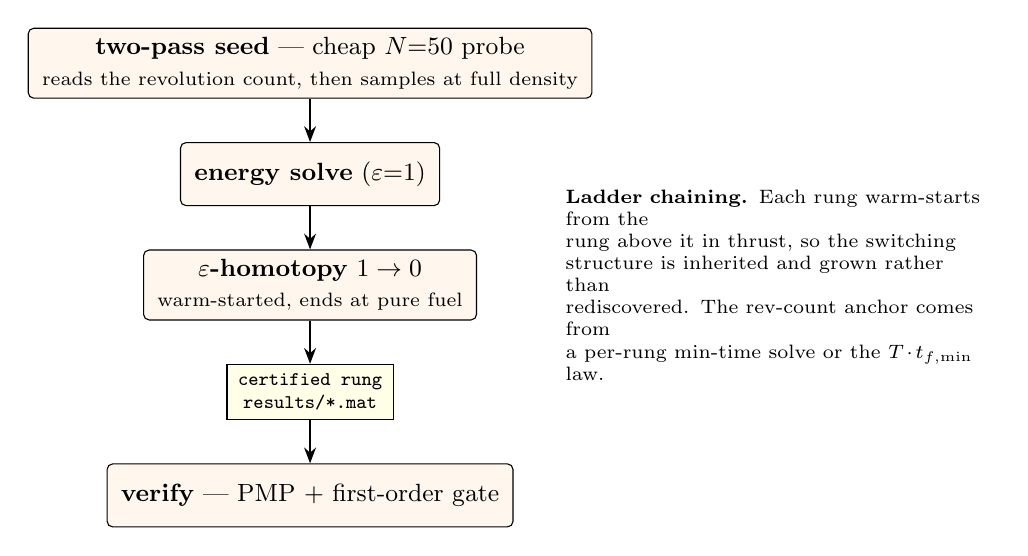
\begin{tikzpicture}[node distance=5.5mm]
  \node[stage] (probe) {\textbf{two-pass seed} --- cheap $N{=}50$ probe\\
       \scriptsize reads the revolution count, then samples at full density};
  \node[stage, below=of probe] (energy) {\textbf{energy solve} ($\varepsilon{=}1$)};
  \node[stage, below=of energy] (hom) {\textbf{$\varepsilon$-homotopy} $1\to0$\\
       \scriptsize warm-started, ends at pure fuel};
  \node[data,  below=of hom] (row) {certified rung\\ \file{results/*.mat}};
  \node[stage, below=of row] (ver) {\textbf{verify} --- PMP + first-order gate};
  \draw[fl] (probe) -- (energy); \draw[fl] (energy) -- (hom);
  \draw[fl] (hom) -- (row); \draw[fl] (row) -- (ver);

  \node[right=10mm of hom, font=\scriptsize, align=left, text width=54mm]
      {\textbf{Ladder chaining.} Each rung warm-starts from the\\
       rung above it in thrust, so the switching\\
       structure is inherited and grown rather than\\
       rediscovered. The rev-count anchor comes from\\
       a per-rung min-time solve or the $T\!\cdot\!t_{f,\min}$ law.};
\end{tikzpicture}
\caption{The per-rung pipeline. The ladder walks
$\SI{10}{\newton}\to\SI{0.1}{\newton}$, chaining rungs.}
\end{figure}

%=======================================================================
\section{How to run it}
%=======================================================================

\begin{lstlisting}[language=Matlab]
cd orbit_transfer/earth_elliptic_to_geo/direct
setup_paths
edit frontdoor/run_gergaud      % set thrustN and endpoints, then run
\end{lstlisting}

\file{run\_gergaud} is the front door: set the thrust and (optionally) custom
endpoints and it produces a Table-3 row, plots and a movie. It has
\texttt{auto}, \texttt{solve} and \texttt{probe} modes.

\begin{lstlisting}[language=bash]
./reproduce_table3.sh           # walk the certified ladder, one process per rung
\end{lstlisting}

\paragraph{Important scope limit.} \file{run\_gergaud} reproduces the shallow
rungs. It will \emph{not} reproduce the deep ladder
($\le\SI{0.5}{\newton}$) --- those need the per-rung recipe registry
(\file{table3\_recipes}), \texttt{liftDL}, and raised iteration caps. The
reasons are documented in \file{doc/campaign\_reproduction\_runbook} §``Why
\file{run\_gergaud} will not reproduce the deep ladder'', and the recipes in
\file{process/DEEP\_THRUST\_LESSONS.md}. Read those before attempting a deep
rung.

%=======================================================================
\section{Status and lessons}
%=======================================================================

\begin{itemize}
\item \textbf{Ladder certified \SI{10}{\newton} $\to$ \SI{0.1}{\newton}.} Final
masses land within the paper's band; $t_{f,\min}$ matches closely.

\item \textbf{\texttt{maxIter} was decisive.} Under-iteration silently collapses
the deep-$\varepsilon$ tail --- the run appears to converge but the switching
structure is not resolved.

\item \textbf{\texttt{scaleNLP} is harmful here}: it fights IPOPT's own
automatic scaling.

\item \textbf{The dual-extraction bug.} \texttt{opti.dual()} returns duals in a
canonicalized constraint orientation; using them directly produced a
primer-vector misalignment of \ang{10} to \ang{60} that resisted explanation
for nine days across two campaigns. The fix is to index
\texttt{opti.lam\_g} by the constraint's own row range. Primer misalignment
went to \ang{0.000} and the sign law to 100\%. Recorded in
\file{process/LESSONS\_DUAL\_EXTRACTION.md}.

\item \textbf{First-order optimality: gated} by the campaign-agnostic layer in
\file{../verify\_common}. \textbf{Second-order: not established.}

\item \textbf{Open:} a $\sim\ang{20}$ dual anomaly at some rungs (escalate
branch), and the \SI{0.5}{\newton} minimum-time wall.
\end{itemize}

%=======================================================================
\section{Companion documents}
%=======================================================================

\begin{center}
\begin{tabular}{ll}
\toprule
document & role \\
\midrule
\file{doc/table3\_method\_note} & the method, in detail \\
\file{doc/campaign\_reproduction\_runbook} & per-rung operational runbook \\
\file{process/DEEP\_THRUST\_LESSONS.md} & the deep-rung recipe \\
\file{process/LESSONS\_DUAL\_EXTRACTION.md} & the \texttt{opti.dual} bug \\
\file{../earth\_elliptic\_to\_geo\_CR3BP/} & the same problem \emph{with} lunar gravity \\
\bottomrule
\end{tabular}
\end{center}

This campaign is the reference pattern for the repository: the CR3BP sibling
extends it by an opt-in third-body branch inside the \emph{shared}
\file{lt\_mee\_rhs.m}, duplicating nothing --- which is why the
\texttt{opti.dual} fix above reached that campaign for free.

\end{document}
